\subsection{Deformational flow on a sphere}

\TODO{how much detail do I need about OpenFOAM's global Cartesian coordinates, lack of 2D meshes and our correction for spherical geometry?}

Tests on cubed sphere and hexagons, again comparing cubicFit against linearUpwind.  \citet{lauritzen2012} had six classes of test and we will reproduce three of them:
\begin{enumerate}
	\item convergence tests with Gaussian hills
	\item minimal resolution test with cosine bell
	\item cosine bell in divergent flow
\end{enumerate}
We will not consider filament preservation, a "rough" distribution with a slotted cylinder, or correlation preservation.

\subsubsection{Numerical order of convergence using Gaussian hills}
\begin{figure}
	\TODO{plot Gaussian hill and cosine bell initial conditions} \\
	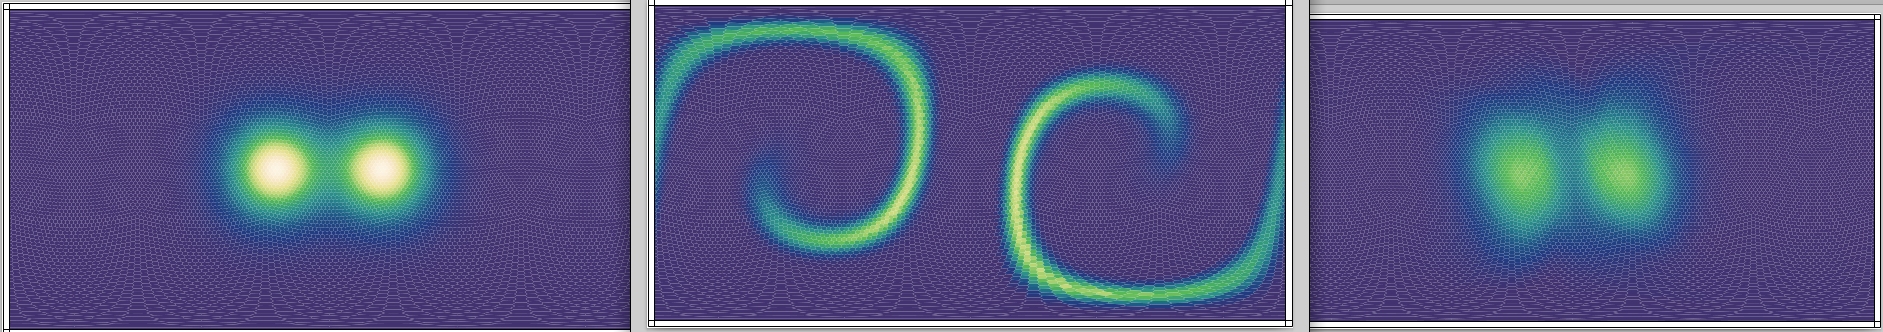
\includegraphics[width=\textwidth]{hexCubUpEvolution.png} \\
	\caption{\TODO{evolution of deformational flow test cases for Gaussian hills with plots at $t=0$, $t=T/2$ and $t=T$.  The analytic solution at $t=T$ is identical to the initial condition.  This figure is supposed to give a sense of what `should' happen, so plot at a high resolution using whichever mesh gives better results.}}
\end{figure}

\begin{figure}
	\includegraphics{../fig-deformationSphere-convergence/fig-deformationSphere-convergence.pdf}
	\caption{\TODO{deformational flow l2 and linf convergence plots comparing cubed sphere and hexagons, cubicFit and linearUpwind.  This figure is comparable to \citet{lauritzen2012} figure 4.}}
\end{figure}

\subsubsection{``Minimal'' resolution using cosine bells}

\begin{figure}
	\caption{\TODO{$\ell_2$ convergence for non-divergent deformational flow using Cosine bells.  Used to find ``minimal'' resolution.  Plot for hexagons and cubed sphere, cubicFit and linearUpwind.  Plot a heavy line for minimal resolution, as in \citet{lauritzen2012} figure 5.}}
\end{figure}

\subsubsection{Transport under divergent flow conditions using cosine bells}

\begin{figure}
	\caption{\TODO{divergent flow at $t=T/2$ and $t=T$ comparing cubed sphere and hexagons, cubicFit and linearUpwind.  Corresponds to \citet{lauritzen2012} figure 9.}}
\end{figure}

